\documentclass[unicode,11pt,a4paper,oneside,numbers=endperiod,openany]{scrartcl}

\usepackage{assignment}
\usepackage{float}

\usepackage{amssymb}

\graphicspath{{./img/}}
\begin{document}

\setassignment
\setduedate{30 October 2019, 11:59pm}

\serieheader{High Performance Computing}{2019}{Student: Gabriel Fernandes de Oliveira}{Discussed with: N/A}{Solution for Assignment 3}{}
\newline

\section*{Parallel Programming with OpenMP }
This assignment begins with the analysis of parallel programs, and
will introduce you to parallel programming using OpenMP. 

\section{Parallel reduction operations using OpenMP \punkte{30}}

\begin{enumerate}

    \item %Implement parallel version of dot product using OpenMP reduction clause.

        My implementation of the dot product using OpenMP reduction clause follows:

        \begin{figure}[H]
            \centering
            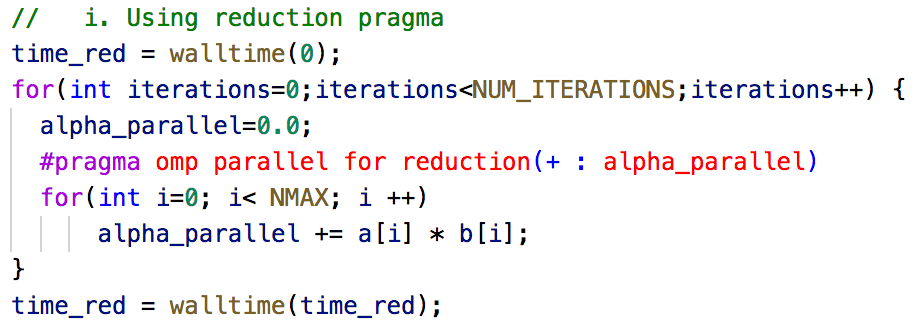
\includegraphics[width=0.9\linewidth]{reduction}
        \end{figure}

        The reduction was created to sum the various multiplications to the variable $alpha\_parallel$.

    \item %Implement parallel version of dot product using OpenMP parallel and critical clauses.

        My implementation of the dot product using OpenMP parallel and critical clause follows:

        \begin{figure}[H]
            \centering
            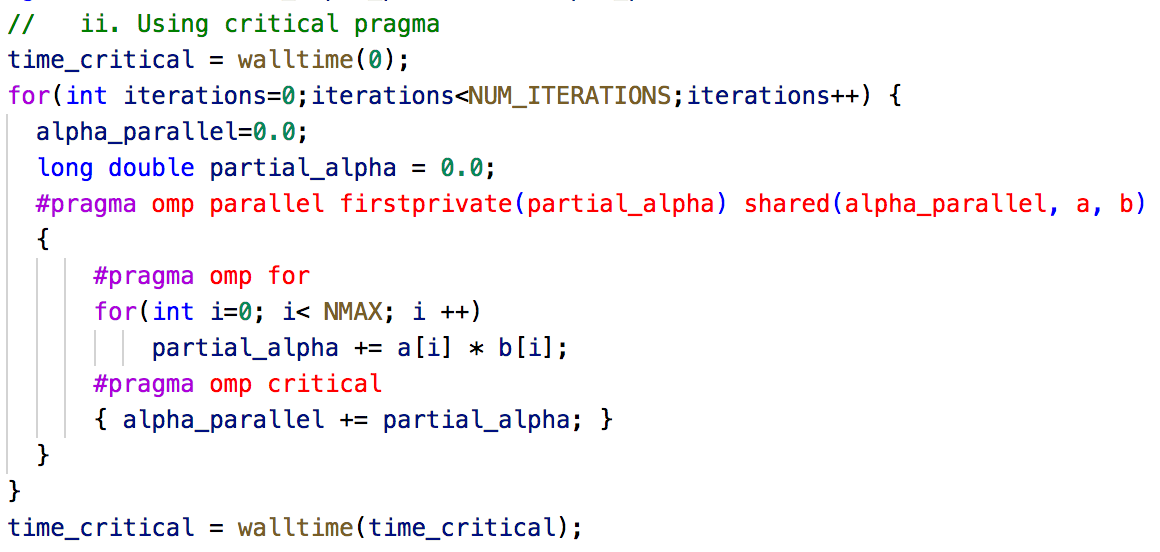
\includegraphics[width=0.9\linewidth]{critical}
        \end{figure}

        To optimize the code, I created an auxiliary variable $partial\_alpha$ that is private for every thread, this helps to reduce the amount of critical sections each thread has to execute.
        
        The only critical section created sums the value of $partial\_alpha$ to the shared variable $alpha\_parallel$. 

    \item %Run the serial and parallel versions on icsmaster cluster, measuring their execution times. Make a performance scaling chart for serial version, parallel version using 1, 2, 4, 8 threads working on vector lengths 100000, 1000000, 10000000, 100000000.

        The first analysis made was plotting the time the dot product takes versus the array sizes:

        \begin{figure}[H]
            \centering
            \includegraphics[width=0.9\linewidth]{"Serial, Reduction and Critical Performance"}
        \end{figure}

        \begin{figure}[H]
            \centering
            \includegraphics[width=0.9\linewidth]{"Serial, Reduction and Critical Performance-2"}
        \end{figure}

        \begin{figure}[H]
            \centering
            \includegraphics[width=0.9\linewidth]{"Serial, Reduction and Critical Performance-3"}
        \end{figure}

        \begin{figure}[H]
            \centering
            \includegraphics[width=0.9\linewidth]{"Serial, Reduction and Critical Performance-4"}
        \end{figure}

    With these graphs it is easy to see the increase in performance the parallel algorithms offer when compared to the serial algorithm. 

    It is also noticeable that the parallel algorithms have a peak in performance at about 4 threads, one can see that there is not much performance gain when using 8 threads.


    To better analyse the performance of the algorithms based on the number of threads I also plotted the following graphs:

        \begin{figure}[H]
            \centering
            \includegraphics[width=0.9\linewidth]{"Serial, Reduction and Critical Performance-5"}
        \end{figure}

        \begin{figure}[H]
            \centering
            \includegraphics[width=0.9\linewidth]{"Serial, Reduction and Critical Performance-6"}
        \end{figure}

        \begin{figure}[H]
            \centering
            \includegraphics[width=0.9\linewidth]{"Serial, Reduction and Critical Performance-7"}
        \end{figure}

        \begin{figure}[H]
            \centering
            \includegraphics[width=0.9\linewidth]{"Serial, Reduction and Critical Performance-8"}
        \end{figure}

        With these graphs it is easier to notice the performance of the parallel algorithms based on the number of threads available.

    \item % In addition to performance scaling, plot the parallel efficiency.

        The following are the graphs of the parallel efficiency for the experiments made.

        The parallel efficiency $E$ was calculated by the formula:
        \[
            E = \frac{t_{seq}}{t_{par}\times num\_threads }
        \]

        Where $t_{seq}, t_{par}$ are the execution times of the serial and parallel algorithms, repectivelly, and $num\_threads$ is the number of the threads available for the experiment

        \begin{figure}[H]
            \centering
            \includegraphics[width=0.9\linewidth]{"Reduction and Critical efficiency"}
        \end{figure}

        \begin{figure}[H]
            \centering
            \includegraphics[width=0.9\linewidth]{"Reduction and Critical efficiency-2"}
        \end{figure}

        \begin{figure}[H]
            \centering
            \includegraphics[width=0.9\linewidth]{"Reduction and Critical efficiency-3"}
        \end{figure}

        \begin{figure}[H]
            \centering
            \includegraphics[width=0.9\linewidth]{"Reduction and Critical efficiency-4"}
        \end{figure}

        Although there is a small variance between the results depending of the array size, the trend in all graphs is the same: the more threads used the worst the efficiency.

        In the previous question we stated that there was no big performance gain from using 4 threads to using 8 threads, the performance in both cases is almost the same.
        This ends up creating a big downgrade in the efficiency value for 8 threads.
        Hence, in all graphs the efficiency for using 8 threads is between $0.25$ and $0.5$.
\end{enumerate}


\section{Visualizing the Mandelbrot Set \punkte{30}}

  %Implement the computation kernel of the Mandelbrot set in the mandel_seq.c. Refer to the pseudo code above.
    The sequential implementation for the computation of the orbit follows: 
    
    \begin{figure}[H]
        \centering
        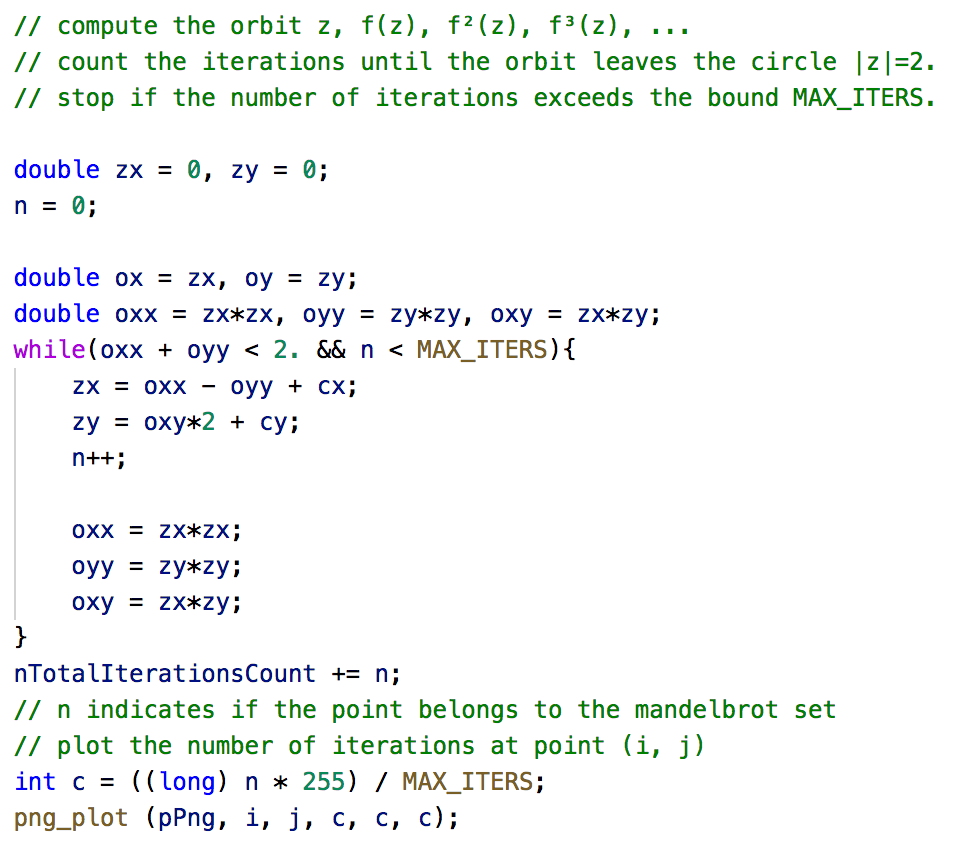
\includegraphics[width=0.9\linewidth]{mandel}
    \end{figure}

    %Count the total number of iterations in order to correctly compute the benchmark statistics. Use the variable nTotalIterationsCount.

    The counting of the total number of iterations is mantained by the variable $nTotalIterationsCount$ which is always incremented by the amount of iterations made in each orbit calculation ($n$).

    The following is the number of iterations required for each image size (using 35207 as the maximum number of iterations on an orbit computation):

    \begin{center}
        \begin{tabular}{||c | c | c | c | c ||} 
            \hline 
            \multicolumn{5}{|c|}{\textbf{Total number of iterations}} \\
            \hline
            256 & 512 & 1024 & 2048 & 4096 \\ [0.5ex] 
            \hline\hline
            444108151 & 1774160381 & 7100090703 & 28390590023 & 113559844217 \\
            \hline
        \end{tabular}
    \end{center}
    




\section{Parallel Mandelbrot \punkte{20}}

    The parallelization process consisted in three main changes:

    \begin{enumerate}

        \item The introduction of the pragma statement.

            \begin{figure}[H]
                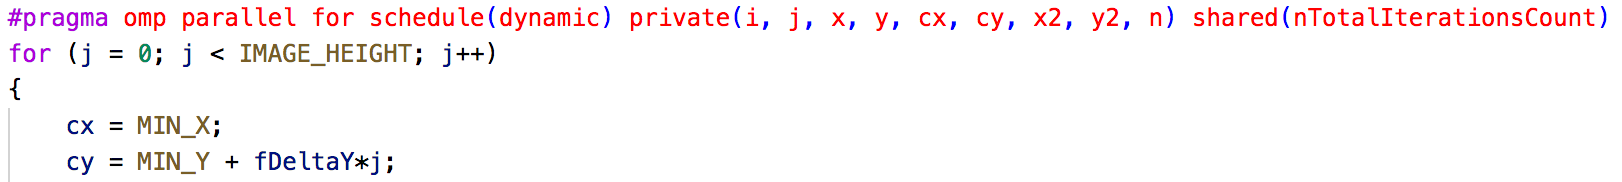
\includegraphics[width=0.9\linewidth]{mandel-par}
                \caption{Lines 36-40 of the file \textit{mandel\_par.c}}
                \label{fig:mandel-par}
            \end{figure}

            I chose to use the dynamic scheduling in order to better divide the work between threads.

            Since it is quite unpredictable if the computation of the orbits will execute $MAX\_ITERS$ iterations or if the loop will be broken in few iterations because the orbit leaves the circle $|z| = 2$, I've decided not to use a static scheduling for the threads.

        \item Changing the way $cy$ was computed.

            In the sequential code $cy$ was initialized with the value $MIN\_Y$ and incremented by $fDeltaY$ after every execution of the loop for the image height (first loop in the mandebrot calculation section).

            In order for this to work in a parallel environment I had to change the way this variable was modified: instead of constantly incrementing the variable I added a line, at the beginning of the loop initializing $cy$ with the value $MIN\_Y + fDeltaY\times j$, as can be seen in figure \ref{fig:mandel-par}.

            Initializing the variable this way removes the need of making $cy$ a shared variable or including a more complicated way to keep track of its value between threads.

        \item Adding a critical section to keep track of the total amount of iterations.

            \begin{figure}[H]
                \centering
                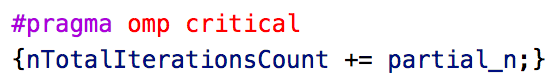
\includegraphics[width=0.7\linewidth]{critical-mandel-par}
                \label{critical-mandel-par}
                \caption{Lines 74-75 of the file \textit{mandel\_par.c}}
            \end{figure}

            Since $nTotalIterationsCount$ is a shared variable, its value must be updated by every thread in a critical section.

            A private variable $partial\_n$ was also created to reduce the amount of critical sections updating the value of $nTotalIterationsCount$.

            

    \end{enumerate}


        I've ran the sequential algorithm and the parallel algorithm with different number of threads and computed the results in the following graphs.

        One can see that the program with 8 threads had a better performance in this problem when comparing to the dot product problem.

            \begin{figure}[H]
                \centering
                \includegraphics[width=0.9\linewidth]{"Sequential and Parallel Mandelbrot set computation"}
            \end{figure}

        The following graph shows very well the performance increase based on the number of threads used.

            \begin{figure}[H]
                \centering
                \includegraphics[width=0.9\linewidth]{"Average time per iteration"}
            \end{figure}

        Doubling the number of threads ended up dividing by half the average time for iteration.


\section{Bug Hunt \punkte{20}}

\begin{itemize}
    \item[\textit{omp\_bug1}]
        This program presents a compile time error.
        That happens because the directive \textit{\#pragma omp parallel for} should be directly followed by a for loop, and this is not what happens in this program.

        In the program, the line following the pragma directive is \textit{tid = omp\_get\_thread\_num()}.

        That explains the compile error the program faces.

        A way to correct this program is the following:

        \begin{figure}[H]
            \centering
            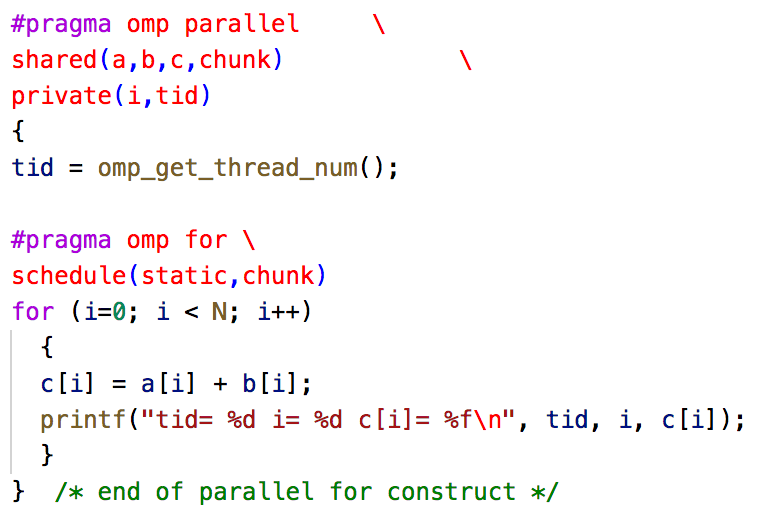
\includegraphics[width=0.9\linewidth]{bug1}
        \end{figure}

        Breaking the pragma in two parts. 
        The first part is just the parallel premisse, without the for and the scheduling part.
        The second part is the for and the desired scheduling strategy, placed right before the for.

    \item[\textit{omp\_bug2}]

        There are two problems in this implementation.

        The first problem is that the messages in the end of the program all claim to be the same thread, this is due to the fact that the variable \textit{tid} is shared through all threads, so the only value displayed at the end is the \textit{id} value of the last thread to execute the line \textit{tid = omp\_get\_thread\_num()}.

        The second problem is in the calculation of the \textit{total} variable, since this variable is shared through all threads its changes should be inside a critical section.
        Instead of using a critical section, one could also use reduction for this for, as shown in the solution that follows:

        \begin{figure}[H]
            \centering
            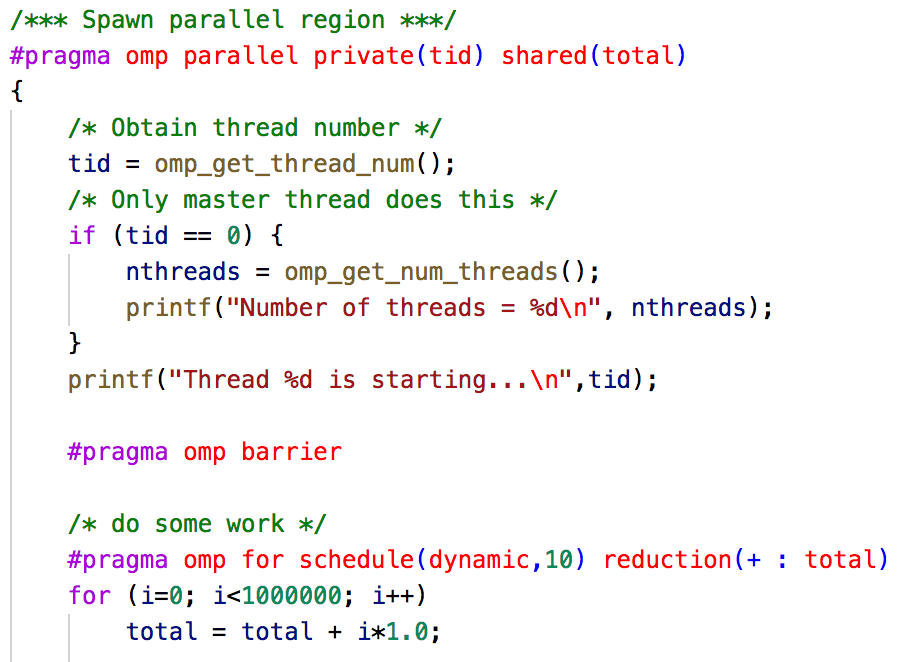
\includegraphics[width=0.9\linewidth]{bug2}
        \end{figure}

        The only necessary changes to solve this remaining problem are making \textit{tid} a private variable and adding the reduction premise before the loop, so that the shared variable \textit{total} will be correctly calculated.

    \item[\textit{omp\_bug3}]

        The main problem here is that the program doesn't end.
        There will always be two threads trapped in the last barrier of the main function, these being the threads that executed the function.

        Follows an illustration of what happens:

        \begin{figure}[H]
            \centering
            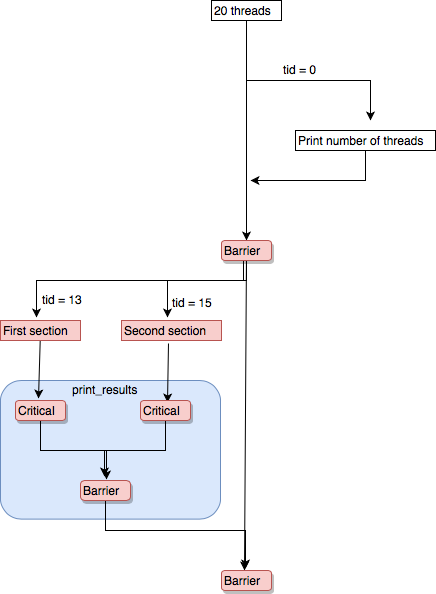
\includegraphics[width=0.9\linewidth]{ThreadFlow}
            \caption{An example of the flow threads may take when executing \textit{omp\_bug3.c}}
            \label{thread-flow}
        \end{figure}

        One can see that two threads, of \textit{tid} 13 and 15 in the example shown in \ref{thread-flow}, pass through three barriers in their flow, whilst all other threads pass through only two barriers.

        This ends up making the threads 13 and 15 stuck on the last barrier, by themselves.
        The program never finishes because the remaining 18 threads the last barrier was waiting for have already been killed since they finished the execution of the main function.

        One possible way to fix this is by removing the extra barrier found in the \textit{print\_results} file.
        This way, all threads synchronize at the end of the function main and finish their execution, allowing the program to end.

        \item[\textit{omp\_bug4}]

            Using \textit{ulimit -a} one can see the stack size that icsmaster allows for usage.
            This value is $8196kB \approx 8.2 MB$.

            In this program the runtime error is caused by a stack memory overflow.
            The matrix $a$ has $1048^2$ doubles, that translates to roughly $8.8MB$.
            Moreover, since $a$ is a private variable, the whole matrix is being copied for every thread created.
            That means that if the program executes with 20 threads, for instance, the memory being used is $20 \times 8.8MB = 175.7MB$ which is much more than the stack can store.

            There are some solutions to this problem:

            \begin{itemize}
                \item 
                    Reducing the dimensions of the matrix to less than $\sqrt{(8.8\times 10^6)/(num\_threads\times 8)}$. 
                    This way, each matrix will have $(8.8\times 10^6)/num\_threads$ doubles.
                    Where $num\_threads$ is the number of threads that will have the matrix as a private variable.

                    This solution would focus on using the maximum memory available.

                \item 
                    The second solution is making $a$ a shared variable, so that it doesn't get copied for every thread.
                    This solves the memory problem, but greatly damages performance, since the updates in the matrix would have to be wrapped by a critical section.

                \item 
                    The final solution, and most clever, would be to simply change the program to remove the matrix $a$, and simply make every thread print the message "Thread $thread-number$ done. Last element=$tid + 2N-2$.

                    This would make the output of the program be the same, improve performance of the routine and also remove the memory problem from the program.
                    But this solution only works because the only element printed by the program is the last one in the matrix, and its calculation is well defined by the program.
            \end{itemize}


        \item[\textit{omp\_bug5}]

            The deadlock caused is very similar to the metaphor for the Dining Philophers.
            There are two resources $a, b$ and two sections that need to use both resources.

            Follows a description of the actions leading to the deadlock, for two threads, named 1 and 2:

            Thread 1 executes the first section and thread 2 executes the second section.

            Thread 1 locks the usage of array $a$ for himself.

            Thread 2 locks the usage of array $b$ for himself.

            Thread 2 tries to lock array $a$ for himself but cannot do it, since it still belongs to thread 1.

            Thread 1 tries to lock array $b$ for himself but cannot do it, since it still belongs to thread 2.

            Hence no thread may advance in their computation, both threads keep infinitelly waiting for each other to release their locks.

            One solution for this problem is changing the order the locks are made. If both threads reserve the usage of $a$ and $b$, in this order, at the beginning of their sections there won't be ny more deadlocks, as implemented in the file \textit{omp\_bug5}.

\end{itemize}

\end{document}
